%%%%%%%%%%%%%%%%%%%%%%%%%%%%%%%%%%%%%%%%%
% a0poster Portrait Poster
% LaTeX Template
% Version 1.0 (22/06/13)
%
% The a0poster class was created by:
% Gerlinde Kettl and Matthias Weiser (tex@kettl.de)
% 
% This template has been downloaded from:
% http://www.LaTeXTemplates.com
%
% License:
% CC BY-NC-SA 3.0 (http://creativecommons.org/licenses/by-nc-sa/3.0/)
%
%%%%%%%%%%%%%%%%%%%%%%%%%%%%%%%%%%%%%%%%%

%----------------------------------------------------------------------------------------
%	PACKAGES AND OTHER DOCUMENT CONFIGURATIONS
%----------------------------------------------------------------------------------------

\documentclass[a0,portrait]{a0poster}

\usepackage{multicol} % This is so we can have multiple columns of text side-by-side
\columnsep=100pt % This is the amount of white space between the columns in the poster
\columnseprule=3pt % This is the thickness of the black line between the columns in the poster

\usepackage[svgnames]{xcolor} % Specify colors by their 'svgnames', for a full list of all colors available see here: http://www.latextemplates.com/svgnames-colors

\usepackage{times} % Use the times font
%\usepackage{palatino} % Uncomment to use the Palatino font

\usepackage{graphicx} % Required for including images
\graphicspath{{figures/}} % Location of the graphics files
\usepackage{booktabs} % Top and bottom rules for table
\usepackage[font=small,labelfont=bf]{caption} % Required for specifying captions to tables and figures
\usepackage{amsfonts, amsmath, amsthm, amssymb} % For math fonts, symbols and environments
\usepackage{wrapfig} % Allows wrapping text around tables and figures

\begin{document}

%----------------------------------------------------------------------------------------
%	POSTER HEADER 
%----------------------------------------------------------------------------------------

% The header is divided into two boxes:
% The first is 75% wide and houses the title, subtitle, names, university/organization and contact information
% The second is 25% wide and houses a logo for your university/organization or a photo of you
% The widths of these boxes can be easily edited to accommodate your content as you see fit

\begin{minipage}[b]{0.75\linewidth}
\veryHuge \color{NavyBlue} \textbf{Cross Translation Unit Analysis in Clang Static Analyzer} \color{Black}\\ % Title
\Huge\textit{ Qualitative Evaluation on C/C++ projects}\\[2cm] % Subtitle
\Large G\'abor Horv\'ath, D\'aniel Krupp, G\'abor M\'arton, Tibor Brunner, P\'eter Sz\'ecsi -- Ericsson \\% Author(s)
\Large Zolt\'an Gera -- E\"otv\"os Lor\'and University\\[0.4cm] % University/organization
\large \texttt{[gabor.a.horvath,daniel.krupp,marton.gabor,tibor.brunner,peter.szecsi]@ericsson.com}\\ \large \texttt{gerazo@elte.hu}\\
\end{minipage}
%
\begin{minipage}[b]{0.25\linewidth}

\includegraphics[width=20cm]{logo.png}\\
\end{minipage}

\vspace{1cm} % A bit of extra whitespace between the header and poster content

%----------------------------------------------------------------------------------------

\begin{multicols}{2} % This is how many columns your poster will be broken into, a portrait poster is generally split into 2 columns

%----------------------------------------------------------------------------------------
%	ABSTRACT
%----------------------------------------------------------------------------------------

\color{Navy} % Navy color for the abstract

\begin{abstract}
Clang Static Analyzer can perform inter-procedural analysis by ''inlining'' 
the callee into the caller's context. This means that the full 
calling context is passed when analyzing the callee and
then the assumptions about the returned value is passed back to the caller. 
This works well for function calls within a
The Cross Translation Unit (CTU) feature allows the analysis of callees
even if the definition of the function is external to the currently 
analyzed TU. This allows detection of bugs in library functions stemming
from incorrect usage (e.g. a library assumes that the user will free a memory 
block allocated by the library), and allows for more precise analysis
of the caller in general if a TU external function is invoked
(by not losing assumptions).

In the CTU analysis mode we usually find 1.5-2 times more potential bugs.
It is of paramount importance to see what are the quality of these reports.
We will examine in detail the following:
\begin{itemize}
\item Identify new true positive and false positive findings.
\item Examine the disappeared findings in detail. Have we lost true positive findings
due to potential coverage loss, or we lost some false positives due 
to more precise analysis?
\item What is the distribution of the path length of the new findings? Reports
with too long (longer than ~15) steps are very hard to understand for a programmer.
\item Evaluate CTU with a new path exploration strategy: prioritize unexplored coverage first \cite{karpenkov}.
\item We evaluate how coverage changes in CTU mode using the different path exploration strategies.
\end{itemize}


\end{abstract}

%----------------------------------------------------------------------------------------
%	INTRODUCTION
%----------------------------------------------------------------------------------------

\color{SaddleBrown} % SaddleBrown color for the introduction

\section*{Introduction}
CTU feature is in upstream Clang since \texttt{https://reviews.llvm.org/rC326323} (Febr 18, 2018)
It can be used by executing tool \texttt{analyze-build --ctu -o reports-ctu} from \texttt{clang/tools/scan-build-py}.


\color{DarkSlateGray} % DarkSlateGray color for the rest of the content

\section*{Qualitative Evaluation on Open Source projects}

We will compare noCTU UFS vs CTU DFS vs CTU UFS .


The following project are analyzed in detail


\begin{enumerate}
\item TMUX
\item CURL
\item Xerces
\end{enumerate}


\begin{center}\vspace{1cm}

\includegraphics[width=0.8\linewidth]{placeholder}
\captionof{figure}{\color{Green} Number of true and false positives}
\end{center}\vspace{1cm}

\begin{center}\vspace{1cm}

\includegraphics[width=0.8\linewidth]{placeholder}
\captionof{figure}{\color{Green} Ratio of true and false positives}
\end{center}\vspace{1cm}

\begin{center}\vspace{1cm}

\includegraphics[width=0.8\linewidth]{placeholder}
\captionof{figure}{\color{Green} Distribution of bug path lengths}
\end{center}\vspace{1cm}


\section*{Ongoing work}

This section reports about ongoing work for shortening bug path length. 

%------------------------------------------------

\subsection*{Bugs in the ASTImporter}

\begin{center}\vspace{1cm}
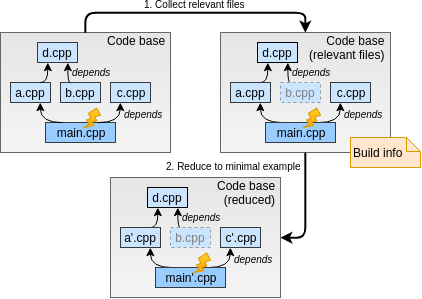
\includegraphics[width=0.8\linewidth]{reducing_process}
\captionof{figure}{\color{Green} Process of ASTImporter failure debugging with 
reducer}
\label{fig:reducing-process}
\end{center}\vspace{1cm}

When an failure is revealed in ASTImporter then it is usually caused by an 
unhandled C/C++ structure or by assembling an invalid AST. Suppose that the 
error happens in \texttt{main.cpp}. Figure \ref{fig:reducing-process} shows the 
debugging process.
\begin{description}
  \item[File collection] Many times we don't have access to the analyzed code 
  base which produces the error. When Clang crashes because of an ASTImporter 
  error, first the files of dependent translation units (i.e. those are 
  containing definitions of referred symbols) are collected recursively 
  together with all the build information which is required to reproduce the 
  error remotely.
  
  \item[Source reduction] In the second phase we use C-Reduce \cite{creduce} to 
  create a minimal version of the code which still produces the error. First 
  the main file is reduced by removing code fragments. If no more code can be 
  removed by providing the same error message, the reduction stops. This 
  process is also accomplished on dependent files.
\end{description}


\subsection*{Shortening Bug Path length}

When the list of bug paths is given then programmers start evaluating the 
results. There are some circumstances which make this process harder. Sometimes 
the length of such a path is about 30 steps and there are also duplicate 
results. Reviewing these is an unnecessary effort.

\begin{center}\vspace{1cm}
  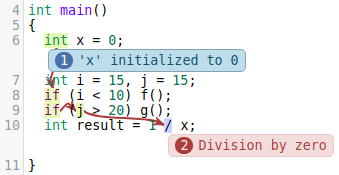
\includegraphics[width=0.5\linewidth]{bugpath}
  \captionof{figure}{\color{Green} Unnecessary bug points}
  \label{fig:bugpath}
\end{center}\vspace{1cm}

Figure \ref{fig:bugpath} shows an example where the \texttt{if} statements are 
part of the bug path, however, these don't take part in the establishment of 
the bug.

We are working on the elimination of the length and number of bug paths by 
three methods:
\begin{itemize}
  \item The irrelevant bug points can be filtered out by a method similar to a 
  slicing algorithm.
  \item Some bug path prefixes can be removed if those don't play role in 
  reaching the final bug point.
  \item Some bug paths are considered the same if they refer the same bug. The 
  number of bugs can be diminished by marking these to be redundant. This will 
  be accomplished by the usage of uniqueing location among multiple translation 
  units.
\end{itemize}


%----------------------------------------------------------------------------------------
%	CONCLUSIONS
%----------------------------------------------------------------------------------------

\color{SaddleBrown} % SaddleBrown color for the conclusions to make them stand out

\section*{Conclusions}

\begin{itemize}
\item Pellentesque eget orci eros. Fusce ultricies, tellus et pellentesque fringilla, ante massa luctus libero, quis tristique purus urna nec nibh. Phasellus fermentum rutrum elementum. Nam quis justo lectus.
\item Vestibulum sem ante, hendrerit a gravida ac, blandit quis magna.
\item Donec sem metus, facilisis at condimentum eget, vehicula ut massa. Morbi consequat, diam sed convallis tincidunt, arcu nunc.
\item Nunc at convallis urna. isus ante. Pellentesque condimentum dui. Etiam sagittis purus non tellus tempor volutpat. Donec et dui non massa tristique adipiscing.
\end{itemize}

\color{DarkSlateGray} % Set the color back to DarkSlateGray for the rest of the content

%----------------------------------------------------------------------------------------
%	REFERENCES
%----------------------------------------------------------------------------------------

\nocite{*} % Print all references regardless of whether they were cited in the 
%%poster or not
\bibliographystyle{plain} % Plain referencing style
\bibliography{sample} % Use the example bibliography file sample.bib

\end{multicols}
\end{document}
